% !TEX TS-program = pdflatex
% !TEX encoding = UTF-8 Unicode

% This is a simple template for a LaTeX document using the "article" class.
% See "book", "report", "letter" for other types of document.

\documentclass[14pt]{article} % use larger type; default would be 10pt

\usepackage[utf8]{inputenc} % set input encoding (not needed with XeLaTeX)

%%% Examples of Article customizations
% These packages are optional, depending whether you want the features they provide.
% See the LaTeX Companion or other references for full information.

%%% PAGE DIMENSIONS
\usepackage{geometry} % to change the page dimensions
\geometry{a4paper} % or letterpaper (US) or a5paper or....
% \geometry{margin=2in} % for example, change the margins to 2 inches all round
% \geometry{landscape} % set up the page for landscape
%   read geometry.pdf for detailed page layout information

\usepackage{graphicx} % support the \includegraphics command and options

% \usepackage[parfill]{parskip} % Activate to begin paragraphs with an empty line rather than an indent
\usepackage{float}
\usepackage{titling}
\setlength{\parindent}{4em}
%%% PACKAGES
\usepackage{booktabs} % for much better looking tables
\usepackage{array} % for better arrays (eg matrices) in maths
\usepackage{paralist} % very flexible & customisable lists (eg. enumerate/itemize, etc.)
\usepackage{verbatim} % adds environment for commenting out blocks of text & for better verbatim
\usepackage{subfig} % make it possible to include more than one captioned figure/table in a single float
% These packages are all incorporated in the memoir class to one degree or another...

%%% HEADERS & FOOTERS
\usepackage{fancyhdr} % This should be set AFTER setting up the page geometry
\pagestyle{fancy} % options: empty , plain , fancy
\renewcommand{\headrulewidth}{0pt} % customise the layout...
\lhead{}\chead{}\rhead{}
\lfoot{}\cfoot{\thepage}\rfoot{}

%%% SECTION TITLE APPEARANCE
\usepackage{sectsty}
\allsectionsfont{\sffamily\mdseries\upshape} % (See the fntguide.pdf for font help)
% (This matches ConTeXt defaults)

%%% ToC(table of contents) APPEARANCE
\usepackage[nottoc,notlof,notlot]{tocbibind} % Put the bibliography in the ToC
\usepackage[titles,subfigure]{tocloft} % Alter the style of the Table of Contents
\usepackage{amsmath}
\renewcommand{\cftsecfont}{\rmfamily\mdseries\upshape}
\renewcommand{\cftsecpagefont}{\rmfamily\mdseries\upshape} % No bold!
\geometry{margin=1.5in}
%%% END Article customizations

%%% The "real" document content comes below...



%\date{} % Activate to display a given date or no date (if empty),
         % otherwise the current date is printed 

\begin{document}
\tableofcontents

\pagebreak
\title{CHAPTER 1}
\maketitle
\section{INTRODUCTION}

\subsection{INTRODUCTION}
         Radar systems are generally used in determining properties, most commonly distance from a reference point, of solid objects using single antennas or large antenna arrays. These antennas transmit and receive electromagnetic signals, which can be processed to obtain various relevant data. By using only one antenna and moving it along a linear axis to record an area of static objects, one can mimic a larger array of antennas to collect high-resolution data: this setup is known as a synthetic aperture radar system. The data collected from this type of radar configuration, after processing, is well-known for its detail and map-like quality, and can be used to render a two-dimensional and three-dimensional representation of scanned area.

\subsection{PROBLEM STATEMENT}
           Radars produce large amounts of data and this has important implications for the archiving and analysis of data. The need for methods to deal with radar data sets will only increase as DRDO is developing multiple sided radar under their project QRSAM. Till now Radar data has been processed in a very traditional manner by going through each bit of big binary files. So, each time whenever an information about particular dwells were needed, it involved a long task of searching each binary files and getting the information. Also the raw radar data contain lot of garbage data which makes it difficult and tedious task to test radar during its development phase. The brute force approach of reading data every time when needed from raw files, uncompressing the data, analysing, loading another chunk, and so on, is impractical. For one, it limits access to the data and prevents parallel research activities.

\subsection{OBJECTIVE}
 To develop a software capable of handling large raw binary radar data and reading each dwells and saving information in a database. Also the software should be capable of reading multiple data without any loss in dwells information and can exclude garbage data. The software should be able to extract clean required radar data and merge it to files. The final objective of this project includes its analysis and the algorithm devised should be fast enough to process large data at real time. 
 
 \pagebreak
 \subsection{STEPS INVOLVED}
 \begin{figure}[H]
  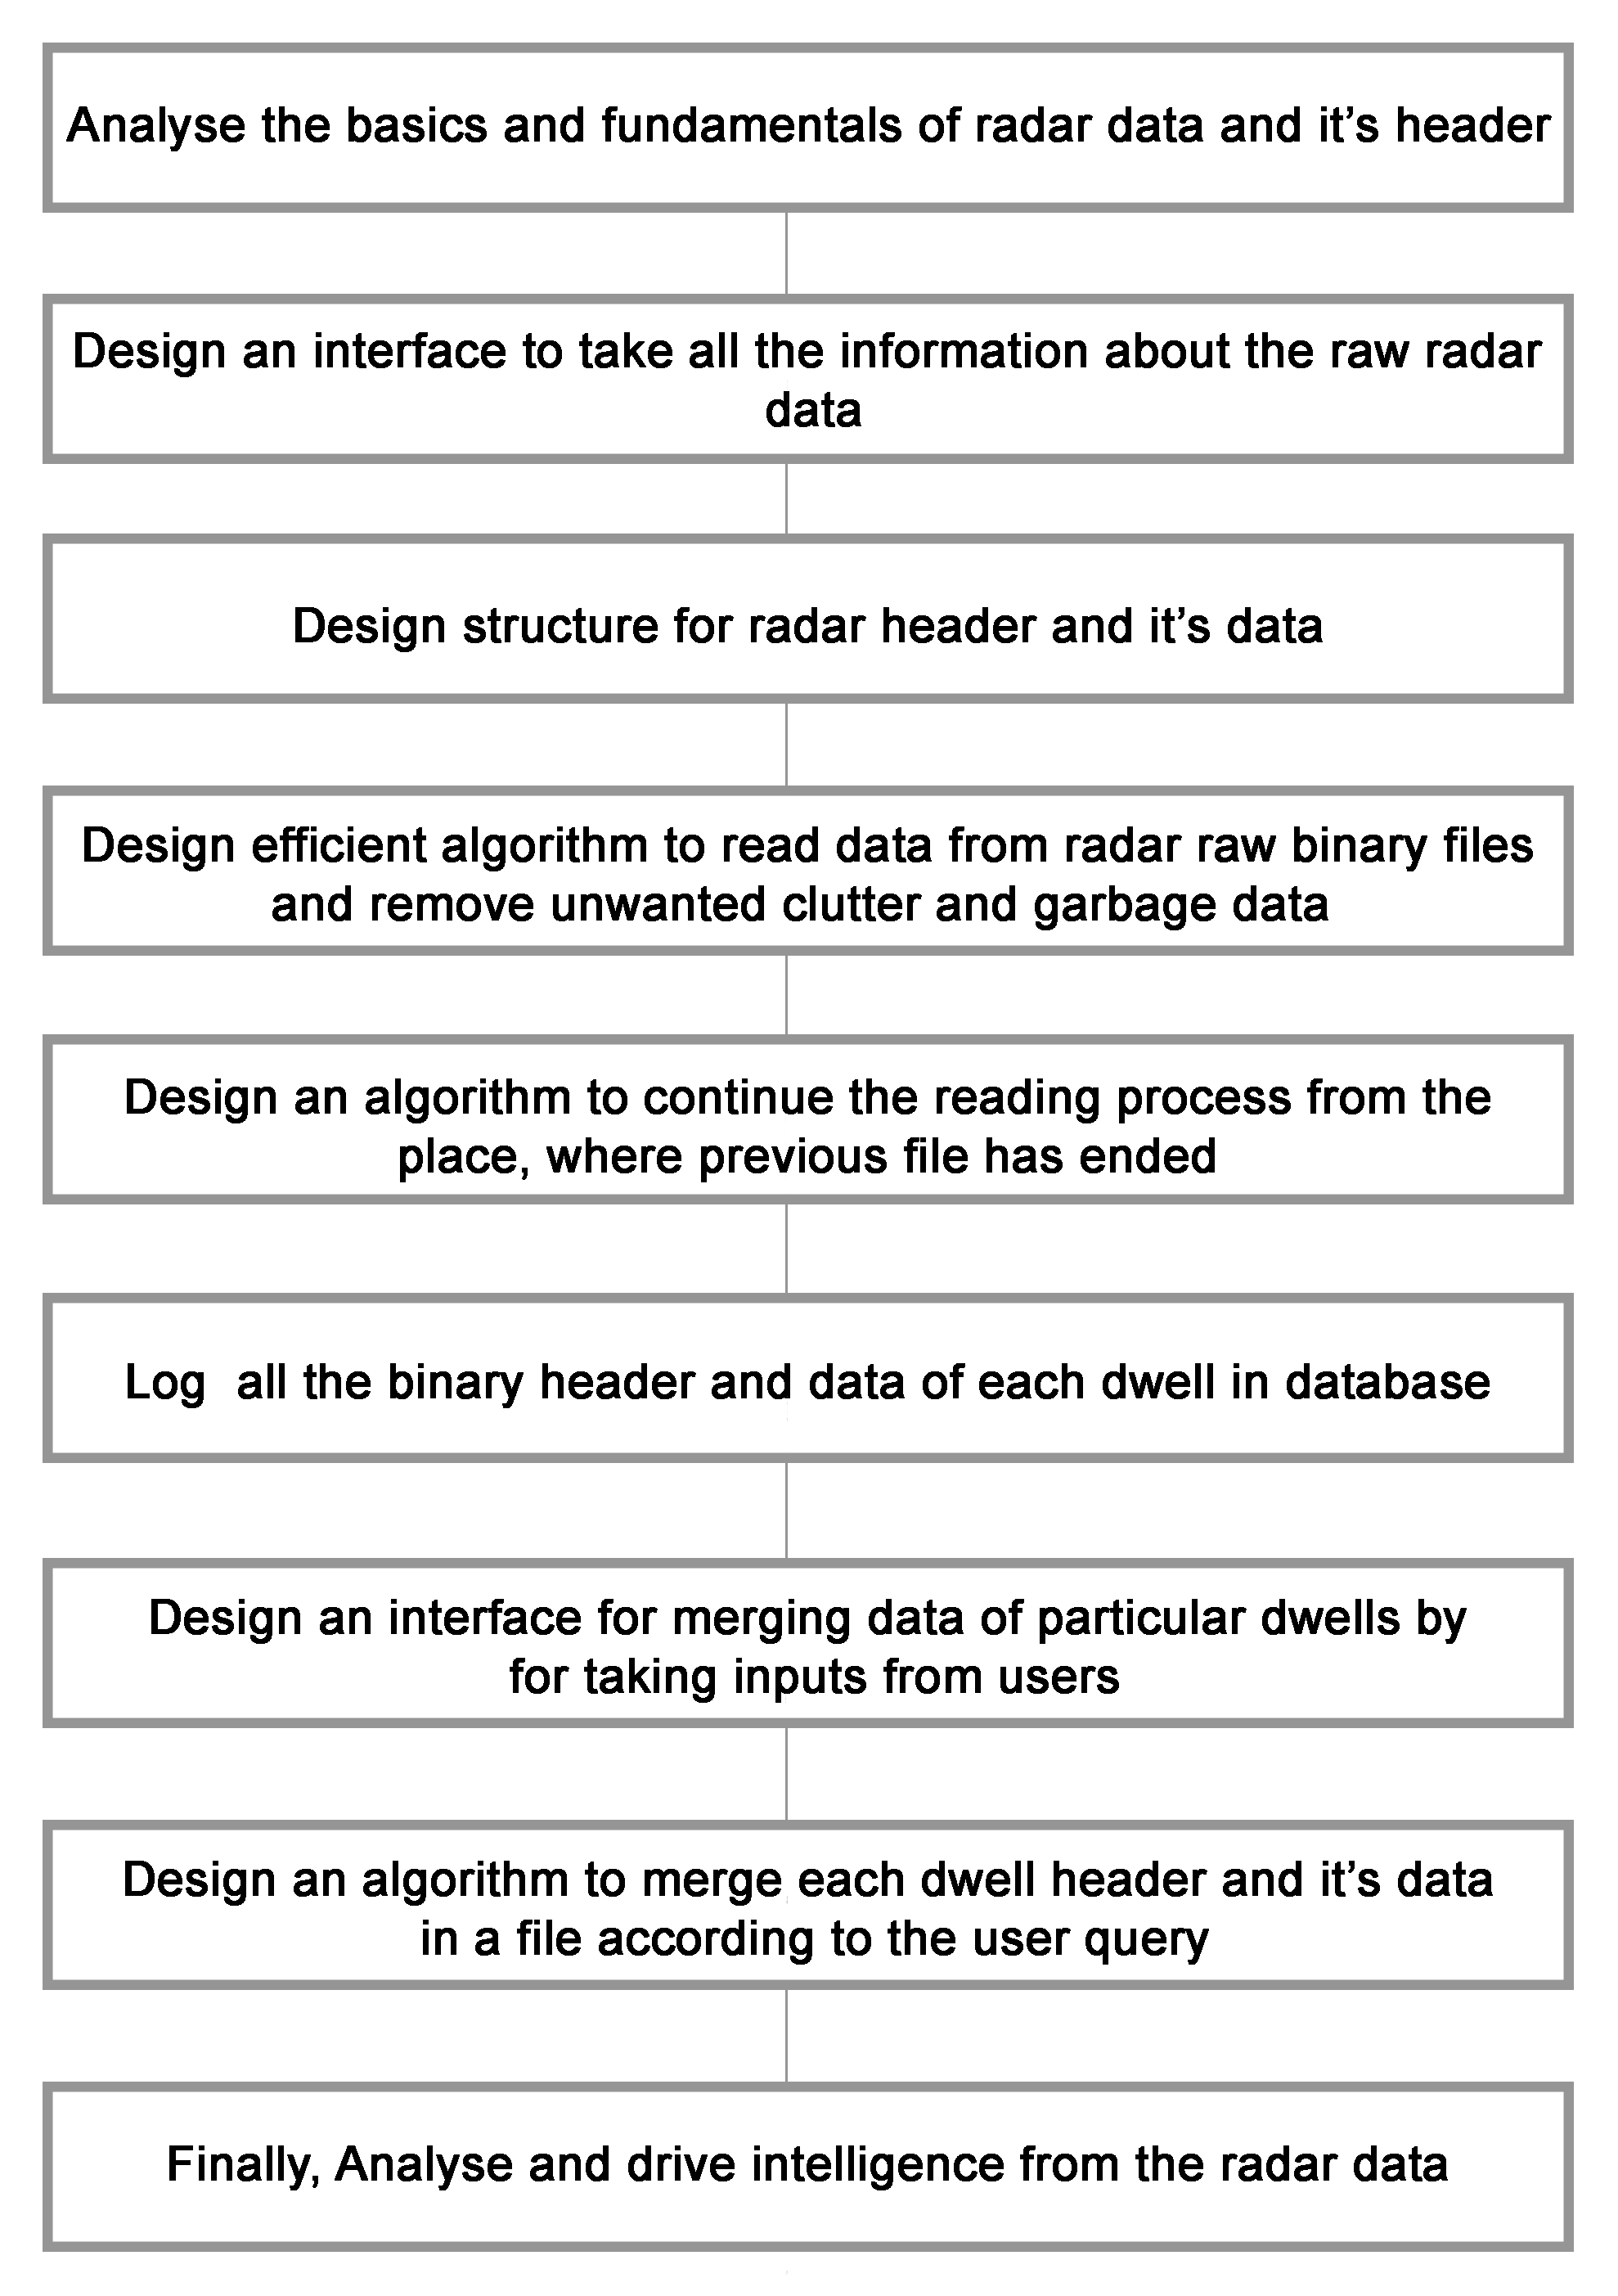
\includegraphics[width=\linewidth]{steps.png}
  \caption{Steps involved.}
  \label{fig:figure 1}
\end{figure}

\subsection{CONSTRAINTS}
Data collected from radars are voluminous. For example, a single volume of radar reflectivity data from the QRSAM, BSR radar requires about   1 GB of disk space. With a volume collected approximately every 30 minutes, this corresponds to 48 GB per day if operated for one day. Archiving and processing such large data sets every time are formidable tasks. The brute force approach of reading data every time when needed from raw files, uncompressing the data, analysing, loading another chunk, and so on, is impractical. For one, it limits access to the data and prevents parallel research activities.

\pagebreak

\title{CHAPTER 2}
\maketitle
\section{ABOUT LRDE, DRDO}

\subsection{ABOUT ORGANISATION}
\textbf{ELECTRONICS AND RADAR DEVELOPMENT ESTABLISHMENT (LRDE)} is one among the labs under \textbf{ Defence Research and Development Organization (DRDO)}. Defence Research \& Development Organisation (DRDO) works under Department of Defence Research and Development of Ministry of Defence. LRDE has its genesis in the Inspectorate of Scientific Stores created in 1939 at  Rawalpindi which was re-designated as Technical Development Establishment (Instruments and Electronics) in 1946 and located at Dehradun. In the year 1958 the Electronics Research and Development Establishment was formed at Bangalore with men and material inherited from TDE (I\&E).. 

\subsection{CORE COMPETENCIES}
\begin{itemize}
 \item	Design and Development of major sub-systems - Mechanical and Electronic Scanning Antennas, High Performance Transmitters, Exciters, Receivers, T/R Modules, Digital Signal \& Data Processors, Mechanical Engineering.
\item	Radar System Engineering for Ground based, Ship borne and Air borne systems.
\item	Environmental engineering including EMI/EMC.
\item	Radar System Integration and Evaluation
\end{itemize}
\subsection{ACTIVITIES}
Design and Development of Radar Systems are
\begin{enumerate}
\item 
\textbf{Army}
\begin{itemize}
\item	Multifunction Phased Array Radar and 3D Surveillance Radar for Akash Missile Weapon System.
\item	 Low Level 2D Radar for Fire Control and Air Defence.
\item	 Short Range Battle Field Surveillance Radar.
\item	 Weapon Locating Radar.
\item	 3D Tactical Control Radar.
	 \end{itemize}
\item
\textbf{Navy}
\begin{itemize}
\item	Maritime Patrol Radar for fixed and Rotary Wing Aircraft.
\item	Maritime Patrol Radar with SAR \& ISAR.
\item	 3D Medium Range Surveillance Radar for ASW Corvettes
\end{itemize}
\item
\textbf{Airforce}
\begin{itemize}
\item	Multifunction Phased Array Radar and 3D Surveillance Radar for Akash Missile Weapon System.
\item	Active Phased Array Radar for AEW\&C.
\item	Low level 2D radar and 3D Short \& Medium Range Surveillance Radar for Air Defence.
\item	Medium Power Radar (MPR).
\item	 Low Level Transportable Radar (LLTR).
\item	Active Electronically Scanned Array Radar (AESA).
\end{itemize}

\end{enumerate}

\pagebreak

\title{CHAPTER 3}
\maketitle
\section{ABOUT RADAR}
\subsection{RADAR FUNDAMENTALS}
Radar is acronym for Radio Detection and Ranging. Radar is an electromagnetic system for detection and location for reflecting objects. Radar can also be used to detect stationary objects buried underground. In some cases, Radar can identify as well .For example, it can identify the type of the aircrafts it has detected. It operates by radiating energy into space and detecting the eco signal reflected from an object or target. The reflected energy that is returned to the radar not only indicates the presence of a target, but by comparing received echo signal with the signal that was transmitted, its location can be determined along with other target related information. Radar can perform its functions at long or short distance and  under conditions improvises to optical and infrared sensors. Its ability to measure distance with high accuracy and weather is one of its most important attributes. The radar makes use of radio waves that are electromagnetic in nature which gets reflected when they encounter some object in their path. 
The time taken by the radio waves to go from the transmitter to the objects and in coming back to the receiver is recorded by Radar, which is used to determine the distance of objects from the Radar by the simple equation given by
 \begin{center}                                             
    R=CT/2
 \end{center}
Where R is range of the target from the Radar.
 C is speed of the electromagnetic wave which is equal to the velocity.
 T is time taken by the pulse to travel from transmitter to target and back from target to receiver.
\subsection{RADAR BLOCK DIAGRAM}
 The block diagram given below Figure 2 shows the main components of the basic radar system and their operations are:
\begin{itemize}

\item \textbf {\underline{Transmitter}:}
\\* The radar transmitter produces the short duration high-power rf pulses of energy that are into space by the antenna.
\item \textbf {\underline{Duplexer}:}
 \\*     The duplexer alternately switches the antenna between the transmitter and receiver so that only one antenna need be used. This switching is necessary because the high-power pulses of the transmitter would destroy the receiver if energy were allowed to enter the receiver.
      
\begin{figure}[H]
  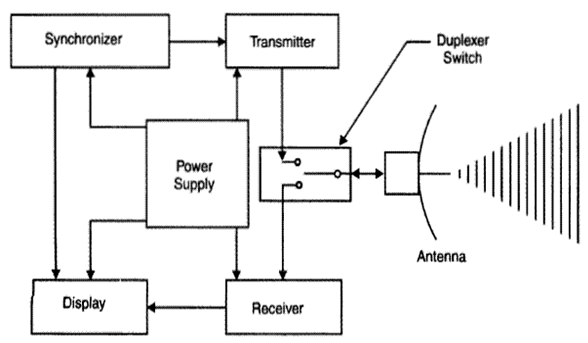
\includegraphics[width=\linewidth]{RadarBlockDiagram.png}
  \caption{Block diagram of radar.}
  \label{fig:figure 2}
\end{figure}


\item \textbf {\underline{Receive}:}
 \\*     The receivers amplify and demodulate the received RF-signals. The receiver provides video signals on the output.
\item \textbf {\underline{Radar-Antenna}:}
 \\*     The Antenna transfers the transmitter energy to signals in space with the required distribution and efficiency. This process is applied in an identical way on reception.
\item \textbf {\underline{Indicator}:}
\\* The indicator should present to the observer a continuous, easily understandable, graphic picture of the relative position of radar targets. The radar screen (in this case a PPI-scope) displays the produced from the echo signals bright blips. The longer the pulses were delayed by the runtime, the further away from the canter of this radar scope they are displayed. The direction of the deflection on this screen is that in which the antenna is currently pointing.
\end{itemize}
\subsection{RADAR FREQUENCY BANDS}
The following Table 1 shows radar frequency bands:

\begin{figure}[H]
  \includegraphics[width=\linewidth]{band.jpg}
  \caption{Radar Frequency Bands}
  \label{fig:figure 3}
\end{figure}
 

High Frequency (HF) radars utilize the electromagnetic waves’ reflection off the ionosphere to detect targets beyond the horizon. Some examples include the United States over the Horizon Backscatter (U.S. OTH/B) radar which operates in the frequency range of, the U.S. Navy Reloadable Over The Horizon Radar (ROTHR), see Fig. 2.3-2, and the Russian Woodpecker radar. Very High Frequency (VHF) and Ultra High Frequency (UHF) bands are used for very long range Early Warning Radars (EWR). Some examples include the Ballistic Missile Early Warning System (BMEWS) search and track mono-pulse radar which operates at (Fig. 2.3-3), the Perimeter and Acquisition Radar (PAR) which is a very long range multifunction phased
array radar, and the early warning PAVE PAWS multifunction UHF phased array radar. Because of the very large wavelength and the sensitivity requirements for very long range measurements, large apertures are needed in such radar systems.


 \begin{figure}[H]
  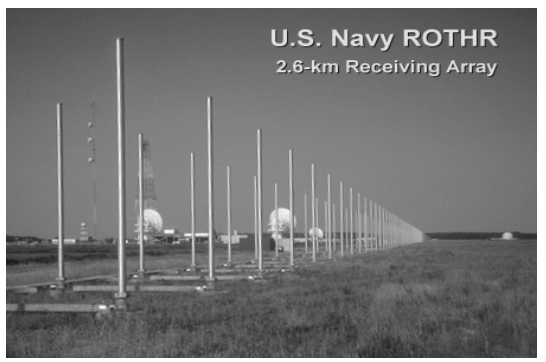
\includegraphics[width=\linewidth]{Horizonradar.png}
  \caption{U. S. Navy Over The Horizon Radar}
  \label{fig:figure 4}
\end{figure}
Radars in the L-band are primarily ground based and ship based systems that are used in long range military and air traffic control search operations. Most ground and ship based medium range radars operate in the S-band. For example, the Airport Surveillance Radar (ASR) used for air traffic control, and the ship based U.S. Navy AEGIS (Fig. 2.6-4) multifunction phased array are S-band radars. The Airborne Warning And Control System (AWACS) shown in Fig. 2.6-5 and the National Weather Service Next Generation Doppler Weather Radar (NEXRAD) are also S-band radars. However, most weather detection radar systems are C-band radars. Medium range search and fire control military radars and metric instrumentation radars are also C-band.


 \begin{figure}[H]
  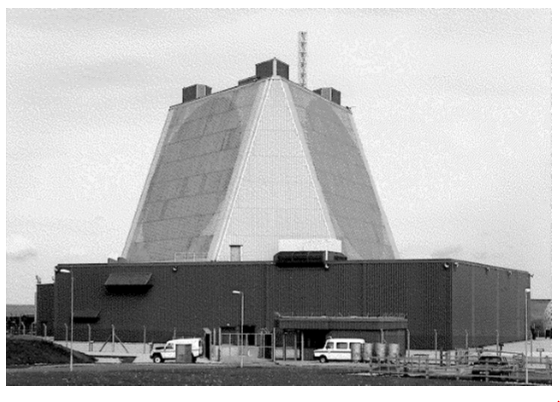
\includegraphics[width=\linewidth]{fylingdales.png}
  \caption{Fylingdales BMEWS - United Kingdom}
  \label{fig:figure 5}
\end{figure}


\begin{figure}[H]
  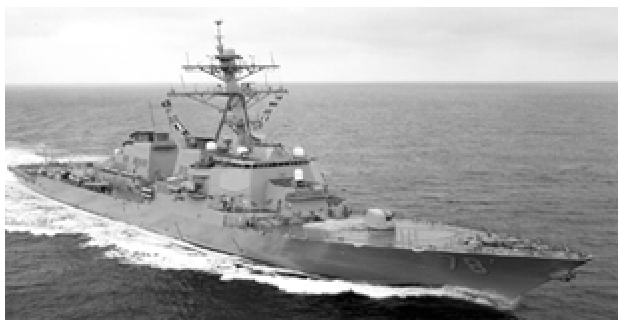
\includegraphics[width=\linewidth]{Navy.png}
  \caption{U. S. Navy AEGIS}
  \label{fig:figure 6}
\end{figure}



 \begin{figure}[H]
  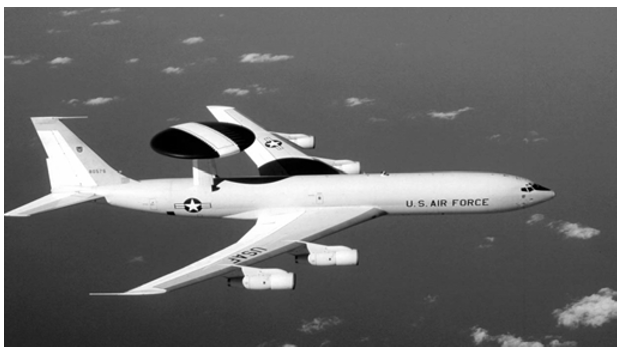
\includegraphics[width=\linewidth]{airforce.png}
  \caption{ U. S. Air Force AWACS}
  \label{fig:figure 7}
\end{figure}

The X-band is used for radar systems where the size of the antenna constitutes a physical limitation; this includes most military multimode airborne radars. Radar systems that require fine target detection capabilities and yet cannot tolerate the atmospheric attenuation of higher frequency bands may also be X-band. The higher frequency bands (Ku, K, and Ka) suffer severe weather and atmospheric attenuation. Therefore, radars utilizing these frequency bands are limited to short range applications, such as the police traffic radars, short range terrain avoidance, and terrain following radars. Milli-Meter Wave (MMW) radars are mainly limited to very short range Radio Frequency (RF) seekers and experimental radar systems.
\subsection{RANGE PERFORMANCE OF RADARS}
The maximum range R\textsubscript{max} equation for radars are:
\[R_{max} = \dfrac{P_tGA_e\sigma}{4\pi^{2}S_{min}} \]

where, \\ \indent P\textsubscript{t} = Transmitted power, in watts,
              \\ \indent G = Antenna gain,
              \\ \indent A\textsubscript{e} = Antenna effective aperture, in m\textsuperscript{2}
                         \\ \indent $\sigma$ =  Radar cross-section of the target, in m\textsuperscript{2}
              \\ \indent S\textsubscript{min} =  Minimum detectable signal, in watts\\


All the above parameters, except $\sigma$  , are to some extent under the control of the radar designer.
\\ In practice, the simple radar equation does not predict the range performance of actual radar equipment’s to a satisfactory degree of accuracy.
 In many cases the actual range might be half of that predicted by the above equation. Some of the major reasons for this are the following:
\begin{itemize} 
\item  Failure of the equation to explicitly include various losses that can occur throughout the system.
\item Loss of performance usually experienced when electronic equipment are operated in the field, as against when they are operated under laboratory conditions.
\item Statistical and unpredictable nature of the various parameters in the radar equation.
\end{itemize}
Both S\textsubscript{min} and $\sigma$ are statistical in nature and must be expressed as such in statistical terms. other statistical factors which affect radar performance are meteorological conditions along the propagation path and performance of the radar operator, if one is employed.
In view of the above, specification of radar range is usually given as the probability that the radar will detect a certain type of target at a particular range.

\subsection{HISTORY OF RADAR}
 Neither a single nation nor a single person can say that the discovery and development of radar technology was his (or its) own invention. One must see the knowledge about “Radar” than an accumulation of many developments and improvements, in which any scientists from several nations took part in parallel. In the past, there are nevertheless some milestones, with the discovery of important basic knowledge and important inventions:
 
\begin{itemize}
\item \textbf {1865  :} The Scottish physicist James Clerk Maxwell presents his “Theory of the Electromagnetic Field” (description of the electromagnetic waves and their propagation) He demonstrated that electric and magnetic fields travel through space in the form of waves, and at the constant speed of light.

\item \textbf {1886 : }The German physicist Heinrich Rudolf Hertz  discovered electromagnetic waves, thus demonstrating the Maxwell theory.

\item \textbf { 1897 :  }The Italian inventor Guglielmo Marconi achieved the first long distance transmission of electromagnetic waves. In his first experiments he used a wire to a wooden pole. In Italian a tent pole is known as lantenna centrale, and the pole with a wire alongside it used as an aerial was simply called lantenna. Today Marconi is known as pioneer of radio communication.

\item \textbf {1900 :  }Nicola Tesla suggested that the reflection of electromagnetic waves could be used for detecting of moving metallic objects.

\item \textbf {1904 :  }The German engineer Christian Hulsmeyer invents the "telemobiloscope" for a traffic monitoring on the water in poor visibility. This is the first practical radar test. Hülsmeyer apply his invention for a patent in Germany, France and the United Kingdom.

\item \textbf {1921 :  }The invention of the Magnetron as an efficient transmitting tube by the US-American physicist Albert Wallace Hull.

\item \textbf {1922 : }The American electrical engineers Albert H. Taylor and Leo C. Young of the Naval Research Laboratory (USA) locate a wooden ship for the first time.

\item \textbf {1930 :  }Lawrence A. Hyland (also of the Naval Research Laboratory), locates an aircraft for the first time.

\item \textbf {1931 : }In Britain the first known proposal for a radar system came from William A. S. Butement and P. E. Pollard in January 1931. They equipped a ship with radar. As antennae were used parabolic dishes with horn radiator. Although their equipment produced short-range results the work was abandoned for lack of government support.

\item \textbf {1933 : }On the basis of the in 1931 from himself invented sonar, Rudolph Kühnhold presented a so called “Funkmessgerat”. It worked on a wavelength of 48 cm and the transmitter had a power of about 40 Watts. From these tests, the Freya-radar was developed, which was produced in series beginning in 1938.

\item \textbf {1935 : } Robert Watson-Watt (later: Sir Robert) suggested that radio waves might be used to detect aircraft at a distance and outlined a means of doing so. Intensive research began and by 1939 Britain possessed a defensive chain of highly secret Radio Direction Finding (RDF) stations.

\item \textbf {1936 :} The development of the Klystron by the technicians George F. Metcalf and William C. Hahn, both General Electric. This will be an important component in radar units as an amplifier or an oscillator tube.

\item \textbf {1939 : }Two engineers from the university in Birmingham, John Turton Randall und Henry Albert Howard Boot built a small but powerful radar using a Multicavity-Magnetron. The B–17 airplanes were fitted with this radar. Now they could find and thus combat the German submarines in the night and in fog.

\item \textbf {1940 :} Different radar equipment’s are developed in the USA, Russia, Germany, France and Japan
.
Driven by general war events and the development of the Air Force to major branch of service, the radar technology undergoes a strong development boost during the World War II, and radar sets were used during the "Cold War" in large numbers along the inner German border.
\end{itemize}

\subsection{ TYPES OF RADAR}
The types of radar are classified into four categories:
\begin{enumerate}
\item	Frequency 
\item	Waveform 
\item	PRF Pulse 
\item	Application
\end{enumerate}

 \begin{figure}[H]
  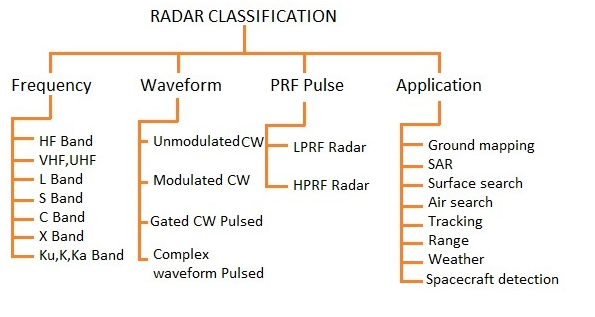
\includegraphics[width=\linewidth]{radartypes.png}
  \caption{ Types of Radar}
  \label{fig:figure 8}
\end{figure}
\subsubsection{Frequency based radar types}
 Following are the radar types based on frequency bands:
 \begin{enumerate}
\item	HF Band Radars
\item	VHF and UHF band radars
\item	L-Band Radars
\item	S-Band Radars 
\item	C-Band Radars 
\item	X-Band Radars 
\item	Ku, K, Ka Band Radars 
\item	Infrared, Visible light band radars
\end{enumerate}

\subsubsection{Waveform Based radar classification}
 Following are the radar types based on waveform:
\begin{enumerate}
\item	Unmodulated CW radar
\item	Modulated CW radar
\item	Gated CW pulsed radar
\item	Complex waveform pulsed radars
\end{enumerate}

\subsubsection{PRF Based radar classification}
Following are the radar types based on PRF:
\begin{enumerate}
\item	LPRF (Low Pulse Repetition Frequency) Radar.
\item	HPRF (High Pulse Repetition Frequency) Radar.
\end{enumerate}

\subsubsection{Application based radar classification}
 Following are the radar types based on their applications of use: 
\begin{enumerate}
\item	Search radars (surface, air)
\item	Warning radars such as weather forecast radars 
\item	Spacecraft detection radars
\item	Fire control radars
\item	Ground mapping radars
\item	SAR 
\item	Air to Surface radars 
\item	Sea surface radar 
\item	Ground moving target search radars 
\item	 Tracking radar
\item	 Range radar
\item	 velocity search radar
\end{enumerate}

\subsection{APPLICATIONS OF RADAR}
Detection and search radar includes the “early warning radar”, used for long-range detection of objects, and the target acquisition(AT), used to locate surface-to-air missiles(SAM).These types are frequently used in the military and in coastal surveillance, as well as for detecting car speed during highway patrol.
Missile guidance system are used to locate the target of a missile. This is often present in military aircraft.
Radar for biological research includes tracking birds and insects to trace their migration patterns. Bird radar is also being used at NASA’s Kennedy space center in Florida to track the presence of birds, especially vultures, near launching pads. Trap and release programs have been implemented to prevent birds accidently impacting the shuttles after lift off.
Air traffic control and navigation radar is used by airports to ensure the safety of planes. This type detects the proximity of an aircraft and identifies the identity and altitude of the plane. Radio beacons and distance measuring equipment(DME) also fall into category.
Weather-sensing radar systems are mostly used to measure and locate precipitation. They can also measure wind direction and speed. 
         Other applications of radar are:
 \begin{enumerate}
\item \textbf {On ground :} Detection, location, and tracking of aircraft and space targets.

\item \textbf {In the air :} Detection of other aircraft, ships, or land vehicles; mapping of land; storm avoidance, terrain avoidance, and navigation.

\item \textbf {On the sea :} Navigation aid and safety device to locate buoys, shore lines, other ships, and for observation of aircraft.

\item \textbf {In space :} Guidance of spacecraft; remote sensing of land and sea.
\newline
\\ \textbf{Some specific applications are as follows:}

\item \textbf {Air traffic control :} Controlling of air traffic in the vicinity of airports; and also for automated landing.

\item \textbf {Aircraft navigation :} Weather avoidance to indicate regions of severe precipitation; terrain following/terrain avoidance (TF/TA); radio altimeter and doppler navigator are also radars.

\item \textbf {Ship safety :} Collision avoidance; detection of navigation buoys.

\item \textbf {Space :} Rendezvous and docking; landing on the moon and other planets; detection and tracking of satellites.

\item \textbf {Remote sensing :} Sensing of geophysical object, or the ”environment” like weather, cloud cover, earth resources, water resources, agriculture, forests, geological formation, etc. This is usually done from aircraft or satellites.

\item \textbf {Law enforcement :} To monitor speed of vehicles in traffic.

\item \textbf {Military :} Surveillance and navigation; control and guidance of weapons. The largest use of radars occurs here.

\end{enumerate}

\subsection{RADAR SUBSYSTEMS}
The following figure 6.3 shows the Product tree of MFR: 

 \begin{figure}[H]
  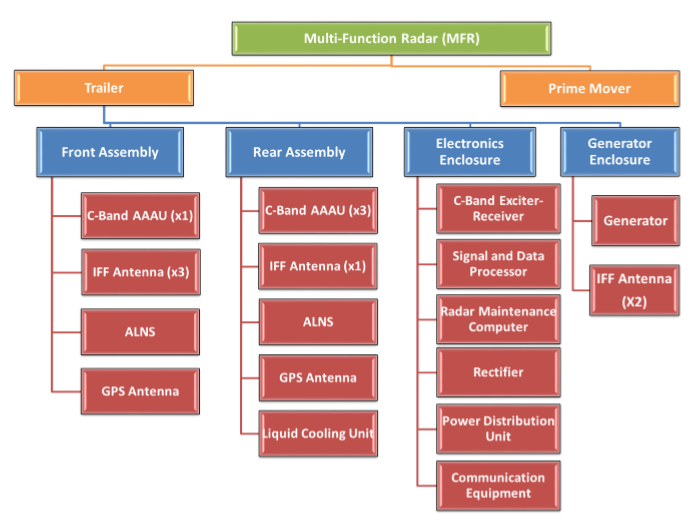
\includegraphics[width=\linewidth]{MFR.png}
  \caption{Product tree of MFR}
  \label{fig:figure 9}
\end{figure}
 \begin{enumerate}
\item \textbf {C-Band Active Array Antenna Unit (AAAU)}
\\The Active Array Antenna Unit (AAAU) consists of the radiating elements array, the Transmit/Receive Modules (TRMs), the power combiner network, the control signal distribution network and the beam steering network. This unit radiates energy in to the coverage volume of interest and collects the echo signals from the environment.
\item \textbf {C-band Exciter-Receiver}  
\\*	This unit consists of the exciter that generates the required RF and timing signals and the receiver which down converts the received echoes.

\item \textbf {Signal and processor}
\\ This unit processes the received signals for Detection, Clutter suppression and parameter extraction are performed by this unit.

\item \textbf {Radar computer}
\\	This subsystem is the brain of the radar and consists of a radar controller, radar data processor, embedded simulator and the interfaces to the external systems. 

\item \textbf {Commander’s console}
\\	The commander’s console consists of a workstation and a display screen and functions as the interface between the operator / commander and the radar.

\item \textbf {Power system}
\\	This consists of a diesel generator, rectifiers and power distribution unit.

\item \textbf {Liquid cooling unit}
\\	This subsystem is responsible for removing heat generated in other subsystems. It consists of a compressor, a pump to circulate a coolant and a heat exchanger.

\item \textbf {Prime Mover with Trailer}
\\	The entire radar system is mounted on this vehicle. The pallet of this vehicle will have a support structure mounted on it which supports all other subsystems.

\item \textbf {Inertial Navigation Unit (INU)}
\\	This subsystem provides the attitudes of the MFR platform.

\item \textbf {IFF unit}
\\	The IFF unit consists of 4 IFF antennas and the IFF interrogator.

\item \textbf {Communication system}
\\       The MFR consists of communication equipment, radio sets and voice communication handsets. MFR will interface with all data communication equipment via gigabit Ethernet. The communication equipment will interact with the external systems via wireless link, with wired link as backup.
	
\item \textbf {AC-DC Rectifier}
\\     The Rectifier receives 415V AC (L-L), 50 Hz, 3Ø power from Diesel Generator (DG) as input and converts it to 320V DC and supplies it to different subsystems.

\end{enumerate}
\end{document}
